\setlength{\parskip}{0.125in}

\chapter{Объявление о проведении Конкурса}

Общество с ограниченной ответственностью <<Мэйл.Ру>>, созданное и действующее в соответствии с законодательством Российской Федерации, с
местом нахождения по адресу: 125167, г. Москва, Ленинградский проспект, д. 39, строение 79, далее по тексту <<Организатор конкурса>>,
приглашает физических лиц, достигших к моменту опубликования настоящего Объявления о конкурсе 18 лет, далее по тексту <<Участник конкурса>>,
к участию в конкурсе на нижеследующих условиях:

\section{Наименование Конкурса}

<<Российский кубок по программированию искусственного интеллекта (Russian AI Cup)>>.

Целями проведения Конкурса являются:
\begin{itemize}
\item повышение общественного интереса к сфере создания программных продуктов;
\item предоставление Участникам конкурса возможности раскрыть творческие способности;
\item развитие профессиональных навыков Участников конкурса.
\end{itemize}

Конкурс состоит из 3 (трёх) этапов, каждый из которых завершается определением Победителей. Последний этап Конкурса является решающим.

\section{Информация об организаторе конкурса}

Наименование: ООО <<Мэйл.Ру>>

Адрес места нахождения: 125167, г. Москва, Ленинградский проспект, д. 39, строение 79

Почтовый адрес: 125167, г. Москва, Ленинградский проспект, д. 39, строение 79, БЦ <<SkyLight>>

Телефон: (495) 725-63-57

Сайт: http://www.russianaicup.ru

Е-мейл: russianaicup@corp.mail.ru

\section{Сроки проведения Конкурса}

Срок проведения Конкурса: с 00.00 часов 7 ноября 2016 года до 24.00 часов 25 декабря 2016 года по Московскому времени.

Первая неделя (с 00.00 часов 7 ноября 2016 года до 24.00 часов 13 ноября 2016 года) и четвёртая неделя (с 00.00 часов 28 ноября 2016 года до
24.00 часов 4 декабря 2016 года) Конкурса являются тестовыми. В течение этого периода функциональность сайта и тестирующей системы Конкурса
может быть неполной, а в правила могут вноситься существенные изменения.

Сроки начала и окончания этапов Конкурса:
\begin{itemize}
\item первый этап – с 00 часов 00 минут 26 ноября 2016 года до 24 часов 00 минут 27 ноября 2016 года;
\item второй этап – с 00 часов 00 минут 10 декабря 2016 года до 24 часов 00 минут 11 декабря 2016 года;
\item третий этап (заключительный) – с 00 часов 00 минут 17 декабря 2016 года до 24 часов 00 минут 18 декабря 2016 года.
\end{itemize}

\section{Условие получения статуса Участника конкурса}

Для участия в Конкурсе необходимо пройти процедуру регистрации в Системе Организатора конкурса, размещённой на сайте Организатора конкурса в
сети Интернет по адресу: http://www.russianaicup.ru.

\section{Срок регистрации Участников конкурса в Системе Организатора}

Регистрация Участников конкурса проводится с 00.00 часов 7 ноября 2016 года до 24.00 часов 25 декабря 2016 года включительно.

\section{Территория проведения Конкурса}

Конкурс проводится на территории Российской Федерации. Проведение всех этапов Конкурса осуществляется путем удалённого доступа к Системе
Организатора конкурса через сеть Интернет.

\section{Условия проведения Конкурса (существо заданий, критерии и порядок оценки)}

Порядок проведения Конкурса, существо задания, критерии и порядок оценки указаны в конкурсной документации в главе 2.

Конкурсная документация включает в себя:
\begin{itemize}
\item Объявление о проведении Конкурса;
\item Соглашение об организации и порядке проведения Конкурса;
\item Правила проведения Конкурса;
\item информационные данные, содержащиеся в Системе Организатора конкурса.
\end{itemize}

Участник конкурса может ознакомиться с конкурсной документацией на сайте Организатора конкурса в сети Интернет по адресу:
http://www.russianaicup.ru, а также при прохождении процедуры регистрации в Системе Организатора конкурса.

Организатор конкурса оставляет за собой право на изменение конкурсной документации, условий проведения Конкурса и отказ от его проведения в
соответствии с условиями конкурсной документации и нормами законодательства РФ. При этом, Организатор Конкурса обязуется уведомить
Участников конкурса обо всех произошедших изменениях путём отправки уведомления, в порядке и на условиях, предусмотренных в конкурсной
документации.

\section{Порядок определения Победителей и вручения Призов. Призовой фонд Конкурса}

Критерии оценки результатов Конкурса, количество и порядок определения Победителей содержатся в главе 2 данного документа.

Призовой фонд Конкурса формируется за счет средств Организатора конкурса.

Призовой фонд:
\begin{itemize}
\item 1 место --- Apple Macbook Pro 13\textquotedbl;
\item 2 место --- Apple Macbook Air 13\textquotedbl;
\item 3 место --- Apple iPad;
\item 4-6 места --- ценные призы;
\item 1-6 места в Песочнице --- ценные призы.
\end{itemize}

Все участники Конкурса, принявшие участие во втором или третьем этапах, будут награждены футболкой. Все участники Конкурса, принявшие
участие в третьем этапе, также получат толстовку с символикой соревнования.

Все участники, занявшие призовые места, будут оповещены посредством отправки сообщения на адрес электронной почты, указанный участником при
регистрации в Системе Организатора.

Призы будут высланы участникам в виде посылок, используя Почту России или другую почтовую службу, в течение двух месяцев после окончания
финального этапа. Срок доставки приза по почтовому адресу, указанному участником, зависит от сроков доставки используемой почтовой службы.
Почтовые адреса призёров для отправки призов Организатор получает из учётных данных участника в Системе Организатора. Адрес должен быть
указан участником-призёром в течение трёх дней после получения уведомления о получении приза.

При отсутствии ответа в обозначенные сроки или отказе предоставить точные данные, необходимые для вручения призов Конкурса, Организатор
оставляет за собой право отказать такому участнику в выдаче приза Конкурса. Денежный эквивалент приза не выдаётся.
 
Победители Конкурса обязуются предоставить Организатору конкурса копии всех документов, необходимых для бухгалтерской и налоговой отчётности
Организатора конкурса. Перечень документов, которые Победитель обязан предоставить Организатору конкурса, может включать в себя:
\begin{itemize}
\item копию паспорта Победителя;
\item копию свидетельства о постановке на налоговый учет Победителя;
\item копию пенсионного удостоверения Победителя;
\item данные об открытии банковского лицевого счета Победителя;
\item иные документы, которые Организатор конкурса потребует от Участника конкурса в целях формирования отчётности о проведённом Конкурсе.
\end{itemize}

Наряду с копиями Организатор конкурса вправе запросить оригиналы вышеуказанных документов.

В соответствии с подпунктом 4 пункта 1 статьи 228 НК РФ Победитель Конкурса, ставший обладателем Приза, самостоятельно несёт все расходы по
уплате всех применимых налогов, установленных действующим законодательством Российской Федерации.

\section{Порядок и способ информирования участников Конкурса}

Информирование Участников Конкурса осуществляется путём размещения информации в сети Интернет на Сайте Организатора конкурса по адресу:
http://www.russianaicup.ru, а также через Систему Организатора конкурса, в течение всего срока проведения Конкурса.

\chapter{О мире CodeWizards 2016}

\section{Общие положения игры и правила проведения турнира}

Данное соревнование предоставляет вам возможность проверить свои навыки программирования, создав искусственный интеллект (стратегию),
управляющий волшебником в специальном игровом мире (подробнее об особенностях мира CodeWizards 2016 можно узнать в следующих разделах).
Правила соревнования базируются на популярном в мире компьютерных игр жанре MOBA. В каждой игре вам будет противостоять пять стратегий
других игроков. В то же время, у вас будет четыре союзника. Пять стратегий, находящиеся на одной стороне, составляют фракцию: Академию или
Отступников. Основной командной целью этих пяти игроков является уничтожение базы противоположной фракции. Основной персональной целью
каждого волшебника является сбор максимально возможного количества баллов. Звание победителя игры, а также все остальные места
распределяются в соответствии с количеством набранных баллов. Два или более игроков могут делить одно место, если их баллы равны. Игроку
начисляются баллы, если его волшебник наносит урон, уничтожает или просто находится рядом во время смерти юнита другой фракции, а также за
некоторые другие действия. Всем игрокам фракции начисляется значительное количество баллов в случае достижения основной командной цели.

Правила игры практически полностью соответствуют классическим канонам жанра. Фракционные базы соединены тремя дорожками (верхней,
центральной и нижней), в промежутках между которыми находятся лесные массивы. На самих дорожках находятся охранные башни: по $2$ на дорожку
от каждой фракции. Таким образом, в начале игры на карте присутствует $14$ строений. С определённым периодом база каждой фракции генерирует
$3$ одинаковых отряда приспешников (<<миньонов>>) волшебников: по одному на каждую дорожку. Они сразу же устремляются по своей дорожке в
направлении базы противоположной фракции, атакуя всех противников на пути.

Турнир проводится в несколько этапов, которым предшествует квалификация в Песочнице. Песочница --- соревнование, которое проходит на
протяжении всего чемпионата. В рамках каждого этапа игроку соответствует некоторое значение рейтинга --- показателя того, насколько успешно
его стратегия участвует в играх.

Начальное значение рейтинга в Песочнице равно $1200$. По итогам игры это значение может как увеличиться, так и уменьшиться. При этом победа
над слабым (с низким рейтингом) противником даёт небольшой прирост, также и поражение от сильного соперника незначительно уменьшает ваш
рейтинг. Со временем рейтинг в Песочнице становится всё более инертным, что позволяет уменьшить влияние случайных длинных серий побед или
поражений на место участника, однако вместе с тем и затрудняет изменение его положения при существенном улучшении стратегии. Для отмены
данного эффекта участник может сбросить изменчивость рейтинга до начального состояния при отправке новой стратегии, включив соответствующую
опцию. В случае принятия новой стратегии системой рейтинг участника сильно упадёт после следующей игры в Песочнице, однако по мере
дальнейшего участия в играх быстро восстановится и даже станет выше, если ваша стратегия действительно стала эффективнее. Не рекомендуется
использовать данную опцию при незначительных, инкрементальных улучшениях вашей стратегии, а также в случаях, когда новая стратегия
недостаточно протестирована и эффект от изменений в ней достоверно не известен.

Начальное значение рейтинга на каждом основном этапе турнира равно $0$. За каждую игру участник получает определённое количество единиц
рейтинга в зависимости от занятого места (система, аналогичная используемой в чемпионате <<Формула-1>>). Если два или более участников делят
какое-то место, то суммарное количество единиц рейтинга за это место и за следующие $\texttt{количество\_таких\_участников}-1$ мест делится
поровну между этими участниками. Например, если два участника делят третье место, то каждый из них получит половину от суммы единиц рейтинга
за третье и четвёртое места. При делении округление всегда совершается в меньшую сторону. Более подробная информация об этапах турнира будет
предоставлена в анонсах на сайте проекта.

Сначала все участники могут участвовать только в играх, проходящих в Песочнице. Игроки могут отправлять в Песочницу свои стратегии, и
последняя принятая из них берётся системой для участия в квалификационных играх. Каждый игрок участвует примерно в одной квалификационной
игре за час. Жюри оставляет за собой право изменить этот интервал, исходя из пропускной способности тестирующей системы, однако для
большинства участников он остаётся постоянной величиной. Существует ряд критериев, по которым интервал участия в квалификационных играх
может быть увеличен для конкретного игрока. Если с момента отправки игроком последней стратегии прошло более недели, то интервал участия
для этого игрока увеличивается вдвое. Учитываются только принятые системой стратегии. За каждое <<падение>> стратегии в $10$ последних
играх в Песочнице начисляется дополнительный штраф, равный $20\%$ от базового интервала тестирования. Подробнее о причинах <<падения>>
стратегии можно узнать в следующих разделах.

Игры в Песочнице проходят по набору правил, соответствующему правилам случайного прошедшего этапа турнира или же правилам следующего
(текущего) этапа. При этом, чем ближе значение рейтинга двух игроков в рамках Песочницы, тем больше вероятность того, что они окажутся в
одной игре. Песочница стартует до начала первого этапа турнира и завершается через некоторое время после финального (смотрите расписание
этапов для уточнения подробностей). Помимо этого Песочница замораживается на время проведения этапов турнира. По итогам игр в Песочнице
происходит отбор для участия в Раунде $1$, в который пройдут $1080$ участников с наибольшим рейтингом (при его равенстве приоритет отдаётся
игроку, раньше отправившему последнюю версию своей стратегии), а также добор в следующие этапы турнира, включая Финал.

Этапы турнира:
\begin{itemize}
  \item В \textbf{Раунде $1$} вам предстоит изучить правила игры и освоить базовое управление волшебником. В каждой игре данного этапа
        примет участие $10$ игроков, которые будут распределены по двум фракциям таким образом, что разница между суммами текущих
        рейтингов\footnote[1]{При проведении игры в рамках Раунда $1$ учитывается рейтинг в нём. При проведении игры в Песочнице по правилам
        Раунда $1$ учитывается рейтинг в Песочнице.} участников двух фракций будет минимальной. Волшебник с наибольшим рейтингом в каждой
        фракции назначается верховным. Его стратегия может отправлять сообщения другим волшебникам из той же фракции, а также ей
        предоставляется больше вычислительных ресурсов (процессорного времени). Функциональность сообщений ограничена и позволяет только
        направлять\footnote[2]{Независимо от этапа турнира, сообщения верховного волшебника могут быть как частично, так и полностью
        проигнорированы стратегиями других волшебников.} других волшебников на определённую линию. В данном режиме волшебникам доступны
        только удар посохом и заклинание <<Магическая ракета>>, а количество жизненной энергии всех строений составляет половину от
        нормального. Коэффициент повреждения при случайном попадании по дружественному волшебнику равен $25\%$. Независимо от этапа
        чемпионата, коэффициент урона по дружественным миньонам и строениям равен нулю. Раунд $1$, как и все последующие этапы, состоит из
        двух частей, между которыми будет небольшой перерыв (с возобновлением работы Песочницы), который позволит улучшить свою стратегию.
        Для игр в каждой части выбирается последняя стратегия, отправленная игроком до начала этой части. Игры проводятся волнами. В каждой
        волне каждый игрок участвует ровно в одной игре. Количество волн в каждой части определяется возможностями тестирующей системы, но
        гарантируется, что оно не будет меньше десяти. $300$ участников с наиболее высоким рейтингом пройдут в Раунд $2$. Также в Раунд $2$
        будет проведён добор $60$ участников с наибольшим рейтингом в Песочнице (на момент начала Раунда $2$) из числа тех, кто не прошёл по
        итогам Раунда $1$.
  \item В \textbf{Раунде $2$} вам предстоит улучшить свои навыки управления волшебником, а также изучить механику получения волшебником
        новых уровней и изучения им умений. Правильный подход к выбору и использованию умений является ключом к победе в данном этапе.
        Компоновка игр осуществляется аналогично Раунду $1$, однако возможности верховного волшебника будут расширены. Он сможет указывать
        другим волшебникам фракции, какие умения им лучше всего изучить. Строения в данном этапе имеют нормальное количество жизненной
        энергии, а коэффициент повреждения при случайном попадании по дружественному волшебнику равен $50\%$. Дополнительно усложняет задачу
        то, что после подведения итогов Раунда $1$ часть слабых стратегий будет отсеяна и вам придётся противостоять более сильным
        соперникам. По итогам Раунда $2$ лучшие $50$ стратегий попадут в Финал. Также в Финал будет проведен добор $10$ участников с
        наибольшим рейтингом в Песочнице (на момент начала Финала) из числа тех, кто не прошёл в рамках основного турнира.
  \item \textbf{Финал} является самым серьёзным этапом. После отбора, проведённого по итогам двух первых этапов, останутся сильнейшие. И в
        каждой игре вам придётся сойтись лицом к лицу с одним из них. Именно так. Для управления пятью волшебниками одной фракции будет
        запущено $5$ экземпляров вашей стратегии. Для управления пятью волшебниками противоположной фракции будет запущено $5$ экземпляров
        стратегии оппонента. В каждой фракции случайный волшебник будет назначен верховным. Он сможет отправлять другим волшебникам фракции
        сообщения в бинарном формате. Ограничение на размер бинарных данных относительно велико, однако получение такого сообщения
        произойдёт после задержки, пропорциональной его длине. Коэффициент повреждения при случайном попадании по дружественному волшебнику
        равен $100\%$. Для определения победителя баллы, набранные всеми волшебниками каждой из фракций, будут просуммированы. В остальном
        правила игры не будут отличаться от правил Раунда $2$. Система проведения Финала имеет свои особенности. Этап по-прежнему делится на
        две части, однако они уже не будут состоять из волн. В каждой части этапа будут проведены игры между всеми парами участников Финала.
        Если позволит время и возможности тестирующей системы, операция будет повторена.
\end{itemize}

После окончания Финала все финалисты упорядочиваются по невозрастанию рейтинга. При равенстве рейтингов более высокое место занимает тот
финалист, чья участвовавшая в Финале стратегия была отослана раньше. Призы за Финал распределяются на основании занятого места после этого
упорядочивания. Лучшие шесть финалистов награждаются призами:
\begin{itemize}
\item 1 место --- Apple Macbook Pro 13\textquotedbl;
\item 2 место --- Apple Macbook Air 13\textquotedbl;
\item 3 место --- Apple iPad;
\item 4-6 места --- ценные призы.
\end{itemize}

После окончания Песочницы все её участники, кроме призёров Финала, упорядочиваются по невозрастанию рейтинга. При равенстве рейтингов более
высокое место занимает тот участник, который раньше отослал последнюю версию своей стратегии. Призы за Песочницу распределяются на основании
занятого места после этого упорядочивания. Лучшие шесть участников Песочницы награждаются ценными подарками.

\section{Описание игрового мира}

Игровой мир является двумерным, а все юниты в нём имеют форму круга. Ось абсцисс в этом мире направлена слева направо, ось ординат ---
сверху вниз, угол $0.0$ совпадает с направлением оси абсцисс, а положительный угол вращения означает вращение по часовой стрелке. Игровая
область ограничена квадратом, левый верхний угол которого имеет координаты ($0.0$, $0.0$), а длина стороны равна $4000.0$. Ни один живой
юнит не может покинуть пределы игровой области.

\newpage
Далее приведена схема карты, где медным цветом обозначены строения Академии (кругом большего радиуса --- база фракции, кругами меньшего
радиуса --- охранные башни), стальным синим цветом --- строения Отступников, зелёным --- деревья. $10$ цветных отметок ($5$ в левом нижнем
углу карты для Академии и $5$ в правом верхнем углу карты для Отступников) являются начальными позициями волшебников. Стоит отметить, что
координаты центров и радиусы деревьев в лесных массивах могут отличаться от игры к игре. Также в процессе игры могут появляться новые
деревья.

Координаты и направления для стратегии, управляющей волшебником Отступников, передаются в преобразованном виде. Таким образом, стратегия
всегда <<думает>>, что её база находится в левом нижнем углу карты, а база противника --- в правом верхнем.

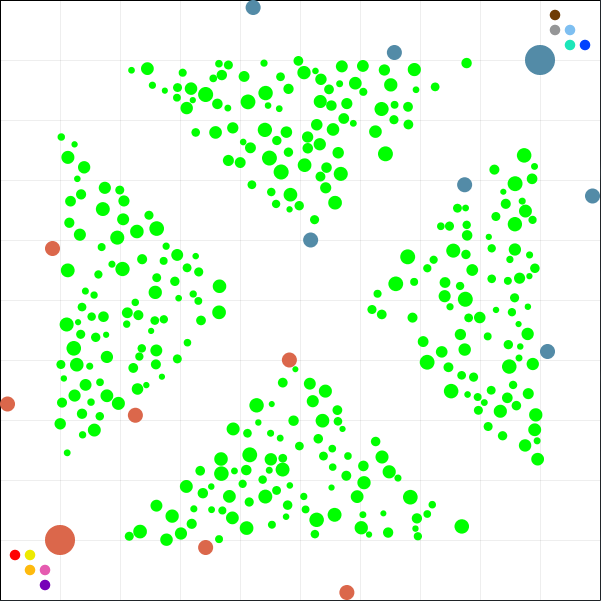
\includegraphics{images/map.png}

Время в игре дискретное и измеряется в <<тиках>>. В начале каждого тика игра получает от стратегий желаемые действия волшебников в этот тик
и обновляет состояние волшебников в соответствии с этими желаниями и ограничениями мира. Затем происходит расчёт изменения мира и объектов в
нём за этот тик, и процесс повторяется снова с обновлёнными данными. Максимальная длительность любой игры равна $20000$ тиков, однако игра
может быть прекращена досрочно, если достигнута командная цель одной из фракций либо стратегии всех участников <<упали>>. Крайне
маловероятно, но всё-таки возможно, что командные цели обеих фракций будут достигнуты в один и тот же тик. Тогда дополнительные баллы
получат все участники игры.

<<Упавшая>> стратегия больше не может управлять волшебником. Стратегия считается <<упавшей>> в следующих случаях:
\begin{itemize}
  \item Процесс, в котором запущена стратегия, непредвиденно завершился, либо произошла ошибка в протоколе взаимодействия между стратегией
        и игровым сервером.
  \item Стратегия превысила одно (любое) из отведённых ей ограничений по времени. Стратегии на один тик выделяется не более $10$ секунд
        реального времени. Но в сумме на всю игру процессу стратегии обычного волшебника выделяется
        \begin{equation}
        20\times\textit{<длительность\_игры\_в\_тиках>}+10000
        \end{equation}
        миллисекунд реального времени и
        \begin{equation}
        10\times\textit{<длительность\_игры\_в\_тиках>}+10000
        \end{equation}
        миллисекунд процессорного времени, а стратегии верховного волшебника
        \begin{equation}
        30\times\textit{<длительность\_игры\_в\_тиках>}+10000
        \end{equation}
        миллисекунд реального времени и
        \begin{equation}
        20\times\textit{<длительность\_игры\_в\_тиках>}+10000
        \end{equation}
        миллисекунд процессорного времени.\footnote[3]{Несмотря на то, что ограничение реального времени заметно выше ограничения
        процессорного времени, запрещено искусственно <<замедлять>> тестирование стратегии командами типа <<\texttt{sleep}>> (равно как и
        пытаться замедлить/дестабилизировать тестирующую систему другими способами). В случае выявления подобных злоупотреблений, жюри
        оставляет за собой право применить к данному пользователю меры на своё усмотрение, вплоть до дисквалификации из соревнования и
        блокировки аккаунта.} В формуле учитывается максимальная длительность игры. Ограничение по времени остаётся прежним, даже если
        реальная длительность игры отличается от этого значения. Все ограничения по времени распространяются не только на код участника, но
        и на взаимодействие клиента-оболочки стратегии с игровым симулятором.
  \item Стратегия превысила ограничение по памяти. В любой момент времени процесс стратегии не должен потреблять более 256 Мб оперативной
        памяти.
\end{itemize}

Обнаружение юнитов на карте ограничено туманом войны. Стратегия участника будет получать данные только о тех юнитах, которые находятся в
пределах дальности\footnote[4]{Здесь и далее под расстоянием между юнитами подразумевается расстояние между их центрами, если явно не
указано другое.} зрения самого волшебника либо любого другого юнита из его фракции.

\section{Классы юнитов}

В мире CodeWizards 2016 существует $6$ классов юнитов, некоторые из которых, в свою очередь, делятся на типы:
\begin{itemize}
    \item волшебники;
    \item снаряды: магическая ракета (\texttt{MAGIC\_MISSILE}), ледяная стрела (\texttt{FROST\_BOLT}), огненный шар (\texttt{FIREBALL}) и
          дротик (\texttt{DART});
    \item бонусы: усиление (\texttt{EMPOWER}), ускорение (\texttt{HASTE}) и щит (\texttt{SHIELD});
    \item строения: база фракции (\texttt{FACTION\_BASE}) и охранная башня (\texttt{GUARDIAN\_TOWER});
    \item миньоны: орк-дровосек (\texttt{ORC\_WOODCUTTER}) и фетиш с дротиками (\texttt{FETISH\_BLOWDART});
    \item деревья.
\end{itemize}

Волшебники, строения, миньоны и деревья являются живыми юнитами. Основными характеристиками каждого живого юнита являются текущее и
максимальное количество жизненной энергии. В общем случае, при падении количества жизненной энергии до нуля юнит считается погибшим и
убирается из игрового мира. Волшебники --- единственные живые юниты, обладающие регенерацией здоровья. Каждый тик они автоматически
восстанавливают некоторое количество жизненной энергии. Скорость регенерации является вещественным числом, как правило, меньшим единицы.
На протяжении нескольких тиков может казаться, что здоровье волшебника не восстанавливается, однако это не так. Суммарная регенерация за
прошедшие тики накапливается в специальном пуле. Волшебник считается погибшим, если целочисленная часть его жизненной энергии падает до
нуля, независимо от того, сколько энергии сейчас накоплено в пуле.

Сравнительные характеристики живых юнитов приведены в следующей таблице:

\begin{tabular}{| l | l | l | l | l | l | l |}
    \hline
    Характеристика живого юнита            & Волшебник             & Орк   & Фетиш & Охранная башня        & База фракции           & Дерево  \\
    \hline
    Радиус                                 & $35$                  & $25$  & $25$  & $50$                  & $100$                  & $20-50$ \\
    Макс. жизн. энергия                    & $100$\footnotemark[5] & $100$ & $100$ & $500$\footnotemark[6] & $1000$\footnotemark[6] & $6-30$  \\
    Дальность зрения                       & $600$                 & $400$ & $400$ & $600$                 & $800$                  & ---     \\
    Дистанция дальнего боя\footnotemark[7] & $500$                 & ---   & $300$ & $600$                 & $800$                  & ---     \\
    Дистанция ближнего боя\footnotemark[8] & $70$                  & $50$  & ---   & ---                   & ---                    & ---     \\
    Интервал между атаками                 & $30$\footnotemark[9]  & $60$  & $30$  & $240$                 & $240$                  & ---     \\
    Урон одной атаки                       & $12$\footnotemark[10] & $12$  & $6$   & $36$                  & $48$                   & ---     \\
    \hline
\end{tabular}

\footnotetext[5]{Максимальная жизненная энергия волшебника нулевого уровня. При получении каждого нового уровня увеличивается на $10$.}
\footnotetext[6]{Реальное количество жизненной энергии строения в конкретном этапе соревнования может отличаться от табличного.}
\footnotetext[7]{Максимальная дальность полёта снаряда либо максимальная дальность между центрами юнитов.}
\footnotetext[8]{Максимально возможная дистанция до ближайшей точки цели.}
\footnotetext[9]{Минимально возможный интервал между двумя последовательными атаками или заклинаниями волшебника. Каждый тип действия
    дополнительно ограничен собственным интервалом.}
\footnotetext[10]{Базовый урон атаки ближнего боя, а также простейшего заклинания <<Магическая ракета>>. Может возрасти вследствие изучения
    волшебником некоторых умений.}

Радиус бонуса, независимо от типа, равен $20$.

Сравнительные характеристики снарядов приведены в следующей таблице:

\begin{tabular}{| l | l | l | l | l |}
  \hline
  Характеристика снаряда    & Магическая ракета & Ледяная стрела & Огненный шар          & Дротик \\
  \hline
  Радиус                    & $10$              & $15$           & $20$                  & $5$    \\
  Скорость                  & $40$              & $35$           & $30$                  & $50$   \\
  Урон при прямом попадании & $12$              & $24$           & $24$\footnotemark[11] & $6$    \\
  \hline
\end{tabular}

\footnotetext[11]{Формально, огненный шар не наносит урона при прямом попадании, однако от столкновения он взрывается, нанося урон всем
    живым юнитам, расстояние от центра огненного шара до ближайшей точки которых не превышает $100$, в том числе и живому юниту, с которым
    произошло столкновение. Если указанное расстояние не превышает радиус огненного шара, то взрыв наносит максимальный урон. По мере
    возрастания дальности урон равномерно уменьшается и на периферии области взрыва составляет половину от табличного.}

Помимо нанесения урона, ледяная стрела дополнительно замораживает (\texttt{FROZEN}) цель на $60$ тиков. Замороженный юнит не может
перемещаться и совершать какие-либо действия, однако количество тиков, оставшееся до применения следующего действия, продолжает уменьшаться.
Здания и деревья не могут быть заморожены. Стратегия волшебника не получает управление до окончания действия заморозки.

При попадании в цель либо при достижении максимальной дальности полёта огненный шар взрывается, нанося урон всем живым юнитам, расстояние от
центра огненного шара до ближайшей точки которых не превышает $100$. При этом на всех юнитов, получивших урон от взрыва, дополнительно
накладывается статус горения (\texttt{BURNING}). Он действует $240$ тиков и за это время наносит $24$ единицы урона. Урон от нескольких
статусов того же типа суммируется.

Атака строения не вызывает создание снаряда. Нанесение урона происходит мгновенно, в результате разряда магической энергии.

Вторая башня на дорожке является неуязвимой до тех пор, пока не уничтожена первая башня на этой дорожке. База фракции может быть атакована
только после того, как на одной из дорожек будут уничтожены обе союзные башни.

\section{Характеристики волшебников}

Основными характеристиками каждого живого юнита являются текущее и максимальное количество жизненной энергии. Однако у волшебника есть ряд
других, не менее важных характеристик. Например, воможность волшебника произносить заклинания ограничена текущим и максимальным количеством
магической энергии, а также скоростью её регенерации.

В отличие от других живых юнитов, волшебника невозможно уничтожить окончательно, можно лишь разрушить его телесную оболочку. Через некоторое
время он возродится в новом теле. Для возрождения должно пройти не менее $1200$ тиков с момента смерти волшебника и не менее $2400$ тиков с
момента последнего его возрождения. Волшебник появляется на своей начальной позиции либо недалеко от неё, если она занята.

В некоторых режимах игры волшебник может накапливать опыт и повышать свой уровень. Начальный уровень каждого волшебника --- нулевой, а
максимальный --- $25$. Тем не менее, правила игры сбалансированы так, что достижение $15$-го уровня является почти невозможной задачей.
Волшебник получает опыт в том же количестве и в тех же случаях, когда игрок, управляющий им, получает баллы, за исключением случаев, когда
волшебник в тик получения баллов мёртв и ожидает возрождения. Для получения первого уровня необходимо набрать $50$ единиц опыта, второго ---
дополнительные $100$ единиц, третьего --- $150$, четвёртого --- $200$ и т.д.

Количество жизненной энергии на нулевом уровне равно количеству магической и составляет $100$ единиц. Прирост количества обоих типов энергии
за каждый уровень равен $10$. Регенерация жизненной энергии на нулевом уровне составляет $0.05$ тиков$^{-1}$ и каждый уровень увеличивается
на $0.005$ тиков$^{-1}$. Соответствующие характеристики магической энергии в $4$ раза выше.

За каждый достигнутый уровень волшебник может изучить ровно одно умение. Умения условно разделены на $5$ групп. Умения внутри каждой группы
имеют строгий порядок, и изучать их можно только последовательно. Количество умений в каждой группе равно $5$. Первое и третье из них, как
правило, пассивно увеличивают одну из характеристик волшебника. Второе и четвёртое являются аурами. Действие ауры аналогично действию
пассивного умения, однако применяется не только к самому волшебнику, но и ко всем дружественным волшебникам, расстояние до которых не
превышает $500$. Если на какого-либо волшебника одновременно действует несколько аур, повышающих одну и ту же характеристику, учитывается
только та из них, которая оказывает наибольший эффект. Последнее, пятое умение в каждой группе является наиболее важным (<<ultimate>>). Оно
позволяет волшебнику произносить новое заклинание либо значительно улучшает уже имеющееся.

\begin{itemize}
    \item Пассивные умения и ауры первой группы увеличивают дальность заклинаний волшебника на $25$ за уровень. Таким образом, дальность
          заклинаний волшебника, изучившего все эти умения, составит $600$. Дополнительно все дружественные волшебники поблизости получат
          прибавку к дальности своих заклинаний, равную $50$. Последнее умение группы позволит использовать заклинание <<Магическая ракета>>
          без задержки. По умолчанию, задержка применения данного заклинания составляет $60$ тиков. Тем не менее, общая задержка на действия
          волшебника всё ещё применяется.
    \item Пассивные умения и ауры второй группы увеличивают урон, наносимый магическими снарядами, на $1$ за уровень. Последнее умение
          группы позволит волшебнику использовать заклинание <<Ледяная стрела>>, которое наносит значительный урон одному противнику, а
          также замораживает его на $60$ тиков.
    \item Пассивные умения и ауры третьей группы увеличивают урон, наносимый при ударе посохом в ближнем бою, на $3$ за уровень. Последнее
          умение группы позволит волшебнику использовать заклинание <<Огненный шар>>, которое наносит урон группе противников, а также
          поджигает их.
    \item Пассивные умения и ауры четвёртой группы увеличивают максимально возможное перемещение волшебника за тик на $5\%$ за уровень.
          Суммарный бонус четырёх умений составит $20\%$, а аура добавит $10\%$ к возможности перемещения дружественных волшебников
          поблизости. Последнее умение группы позволит волшебнику использовать заклинание <<Ускорение>>, которое применяет к дружественному
          волшебнику статус \texttt{HASTENED} на $600$ тиков. Данный статус добавляет дополнительные $30\%$ к скорости перемещения, а также
          увеличивает скорость поворота на $50\%$. Действие нескольких статусов того же типа не суммируется.
    \item Пассивные умения и ауры пятой группы уменьшают урон, получаемый от магических снарядов и атак строений, на $1$ за уровень.
          Последнее умение группы позволит волшебнику использовать заклинание <<Щит>>, которое применяет к дружественному волшебнику статус
          \texttt{SHIELDED} на $600$ тиков. Данный статус уменьшает любой прямой урон на $25\%$. Исключение составляет только урон от
          статуса \texttt{BURNING}. Действие нескольких статусов того же типа не суммируется.
\end{itemize}

Полный список доступных умений вы можете найти в документации к перечислению \texttt{SkillType} (глава 4).

\section{Управление волшебником}

В начале каждого тика симулятор игры отправляет стратегии каждого живого волшебника сведения о текущем состоянии видимой этому волшебнику
части мира. В ответ стратегия отправляет набор инструкций для управления волшебником, инкапсулированных в объекте класса \texttt{Move}.

Эти инструкции обрабатываются в следующем порядке:
\begin{itemize}
    \item Каждый волшебник изучает умение \texttt{move.skillToLearn}, если оно установлено. Игровой симулятор проигнорирует инструкцию,
          если количество изученных волшебником умений уже равно его уровню либо волшебник ещё не изучил все предшествующие умения в группе.
    \item Затем волшебники в случайном порядке совершают действия, установленные в \texttt{move.action}:
          \begin{itemize}
              \item \texttt{NONE}. \textit{Ничего не делать.}
              \item \texttt{STAFF}. \textit{Ударить посохом.} Атака поражает все живые объекты, центр которых находится в секторе от
                    $-\pi / 12$ до $\pi / 12$. Расстояние от центра волшебника до ближайшей точки цели не должно быть больше $70$. Если
                    волшебник погиб в результате удара посохом другого волшебника, совершённого ранее в этот же тик, то удар посохом всё
                    равно будет произведён. Погибший волшебник не приобретёт опыта за нанесённый урон, однако игрок, чья стратегия управляет
                    этим волшебником, получит соответствующее количество баллов.
              \item \texttt{MAGIC\_MISSILE}, \texttt{FROST\_BOLT} или \texttt{FIREBALL}. \textit{Создать соответствующий магический снаряд.}
                    При создании снаряда его центр совпадает с центром волшебника, а направление определяется как
                    \texttt{wizard.angle + move.castAngle}. Значение \texttt{move.castAngle} устанавливается стратегией и ограничено
                    интервалом от $-\pi / 12$ до $\pi / 12$. Дополнительные параметры \texttt{move.minCastDistance} и
                    \texttt{move.maxCastDistance} определяют минимальную и максимальную дальность полёта снаряда. Если расстояние от центра
                    снаряда до точки его появления меньше, чем \texttt{move.minCastDistance}, то снаряд беспрепятственно проходит сквозь все
                    другие игровые объекты, за исключением деревьев. Если расстояние от центра снаряда до точки его появления больше, чем
                    \texttt{move.maxCastDistance}, то снаряд убирается из игрового мира. При этом, снаряд типа \texttt{FIREBALL} детонирует.
                    Столкновения магического снаряда и создавшего его волшебника игнорируются. Если волшебник погиб в результате удара
                    посохом другого волшебника, совершённого ранее в этот же тик, то снаряд создан не будет.
              \item \texttt{HASTE} или \texttt{SHIELD}. \textit{Применить к цели соответствующий магический статус.} Статус применяется к
                    дружественному волшебнику с идентификатором \texttt{move.statusTargetId} или к самому себе, если такой волшебник не
                    найден. Цель должна находиться в секторе от $-\pi / 12$ до $\pi / 12$, а расстояние до неё не должно превышать
                    \texttt{wizard.castRange}. Значение \texttt{wizard.castRange} для волшебника нулевого уровня равно $500$, однако может
                    возрасти до $600$ после изучения некоторых умений. Если волшебник погиб в результате удара посохом другого волшебника,
                    совершённого ранее в этот же тик, статус не будет применён.
          \end{itemize}

          Между любыми двумя последовательными действиями волшебника, отличными от \texttt{NONE}, должно пройти не менее $30$ тиков. Каждому
          действию также соответствует своя собственная задержка, которая ограничивает последовательное использование двух действий одного
          типа. Создание снаряда или применение статуса расходует магическую энергию волшебника. Желаемое действие будет проигнорировано,
          если её недостаточно.

          \begin{tabular}{| l | l | l | l |}
              \hline
              Характеристика действия & Удар посохом & Ускорение & Щит   \\
              \hline
              Задержка                & $60$         & $120$     & $120$ \\
              Стоимость               & ---          & $48$      & $48$  \\
              \hline
          \end{tabular}

          \begin{tabular}{| l | l | l | l |}
              \hline
              Характеристика действия & Магическая ракета     & Ледяная стрела & Огненный шар \\
              \hline
              Задержка                & $60$\footnotemark[12] & $90$           & $120$        \\
              Стоимость               & $12$                  & $36$           & $48$         \\
              \hline
          \end{tabular}
    \item Далее волшебники снова упорядочиваются случайным образом, и происходит их перемещение.

          В мире CodeWizards 2016 нет инерции, и изменение скорости происходит мгновенно. Пожелание стратегии \texttt{move.speed} определяет
          перемещение волшебника вперёд/назад, а \texttt{move.strafeSpeed} --- перемещение боком. Значение \texttt{move.speed} ограничено
          интервалом от $-3.0$ до $4.0$, где положительные значения соответствуют движению вперёд, а отрицательные --- назад. Значение
          \texttt{move.strafeSpeed} ограничено интервалом от $-3.0$ до $3.0$, где положительные значения соответствуют движению правым
          боком, а отрицательные --- левым. Границы обоих интервалов могут быть расширены в зависимости от изученных волшебником умений, от
          действия некоторых аур, а также в случае действия статуса \texttt{HASTENED}. Оба типа перемещения могут осуществляться
          одновременно в один тик, однако в таком случае к ним применяется дополнительное ограничение: если значение
          \texttt{$\sqrt{(\frac{move.speed}{maxSpeed})^2 + (\frac{move.strafeSpeed}{maxStrafeSpeed})^2}$} больше $1.0$, то обе установки
          скорости перемещения (\texttt{move.speed} и \texttt{move.strafeSpeed}) будут поделены игровым симулятором на это значение.
          \texttt{maxSpeed} и \texttt{maxStrafeSpeed} --- соответствующие ограничения, действующие на перемещение волшебника в данный тик (с
          учётом направления перемещения, изученных умений и действующих аур и статусов).

          Перемещение волшебников осуществляется последовательно, согласно выбранному порядку. При этом, частичное перемещение волшебника не
          применяется. Если позицию волшебника невозможно изменить на всю величину указанного стратегией перемещения\footnotemark[13], то
          его перемещение откладывается. После окончания перебора игровой симулятор снова итерируется по всем волшебникам и пытается
          переместить тех, чья позиция в данный тик ещё не изменялась. Так происходит до тех пор, пока не будут перемещены все волшебники.
          Если на очередной итерации не было перемещено ни одного волшебника, то операция также прерывается.

    \item Все волшебники поворачиваются на указанный стратегией угол. По умолчанию, модуль угла поворота волшебника ограничен значением
          $\pi / 30$. Статус \texttt{HASTENED} увеличивает скорость поворота в $1.5$ раза.
\end{itemize}

\footnotetext[12]{Задержка применения заклинания <<Магическая ракета>> может быть ниже в результате изучения некоторых умений.}
\footnotetext[13]{Волшебник после перемещения частично или полностью находится за пределами карты либо пересекается с каким-либо другим
    живым юнитом.}

Помимо выше перечисленных действий, верховный волшебник может отправлять сообщения другим волшебникам из своей фракции. Поле
\texttt{message.lane} содержит рекомендацию отправляться на соответствующую дорожку. Поле \texttt{message.skillToLearn} становится доступным
в Раунде $2$ и содержит рекомендацию изучить указанное умение. Умение может требовать предварительного изучения других умений или быть
недоступно для изучения в данный момент в связи с низким уровнем волшебника. Волшебнику рекомендуется запомнить указание и двигаться в
направлении его реализации. При этом, более позднее указание должно считаться более приоритетным. В Финале у верховного волшебника
появляется возможность отправлять текстовые сообщения. Поле \texttt{message.rawMessage} является массивом байт, а его максимальная длина
равна $1024$. Обычно волшебники получают сообщения на следующий тик после отправки, однако при наличии текстовой части момент получения
сообщения будет отложен на \texttt{ceil(message.rawMessage.length / 2.0)} игровых тиков. Если в системе уже зарегистрировано сообщение для
какого-либо волшебника, но ещё им не получено, то новые сообщения этому волшебнику будут проигнорированы.

\section{Другие игровые объекты}

Каждые $750$ тиков база каждой фракции генерирует $3$ отряда миньонов: по одному на каждую дорожку. Каждый такой отряд состоит из трёх орков
и одного фетиша. Отряд сразу же устремляется по своей дорожке в направлении базы противоположной фракции, атакуя всех противников на пути.
Волшебники используют миньонов как пушечное мясо. При этом сами они стараются держаться в безопасной зоне и атакуют противника на
расстоянии.

В лесных зонах с некоторой вероятностью могут появляться нейтральные миньоны. Обычно они не агрессивны, однако в случае нанесения урона
одному из них все нейтральные миньоны поблизости устремляются к обидчику, атакуя при этом любого, кто встанет у них на пути.

Миньоны могут перемещаться вперёд со скоростью $3$ тика$^{-1}$ и поворачиваться за один тик на угол, не превышающий $\pi / 30$.

Каждые $2500$ тиков на карте может появиться до двух бонусов: в точках $(1200, 1200)$ и $(2800, 2800)$. Если любая часть области появления
бонуса уже занята волшебником или другим бонусом, то создание бонуса будет отложено до окончания очередного интервала.

\section{Столкновения юнитов}

\begin{itemize}
  \item Коллизия живых юнитов между собой, а также с границами карты не допускается игровым симулятором.
  \item Если расстояние от центра живого юнита до центра снаряда меньше или равно сумме их радиусов, то живой юнит получает урон, а снаряд
        убирается из игрового мира. При этом, огненный шар взрывается и наносит урон всем живым юнитам, находящимся поблизости.
  \item Если расстояние от центра волшебника до центра бонуса меньше или равно сумме их радиусов, то волшебник на $2400$ тиков приобретает
        магический статус, в зависимости от типа бонуса:
        \begin{itemize}
            \item \texttt{EMPOWER} в $1.5$ раза увеличивает урон, наносимый волшебником при ударах посохом и попаданиях магических снарядов
                  в цель.
            \item \texttt{HASTE} ускоряет перемещение волшебника, аналогично одноимённому заклинанию.
            \item \texttt{SHIELD} уменьшает урон, получаемый волшебником, аналогично одноимённому заклинанию.
        \end{itemize}
\end{itemize}

Все типы столкновений, не описанные в данном документе, игнорируются игровым симулятором.

\section{Начисление баллов}

Волшебник получает опыт в том же количестве и в тех же случаях, когда игрок, управляющий им, получает баллы, за исключением случаев, когда
волшебник в тик получения баллов мёртв и ожидает возрождения. Баллы начисляются за следующие дествия:
\begin{itemize}
    \item Нанесение повреждений зданиям или волшебникам противоположной фракции. Повреждения учитываются с коэффициентами $0.5$ и $0.25$
        соответственно. Округление производится вниз до ближайшего целого числа. Баллы за повреждения начисляются только тому игроку,
        волшебник которого нанёс эти повреждения.
    \item Уничтожение зданий или волшебников противоположной фракции, а также миньонов любой фракции, отличной от фракции волшебника.
        Суммарное вознаграждение за здания составляет $50\%$ от максимального количества их жизненной энергии, за миньонов --- $25\%$, за
        волшебников --- $100\%$. Уничтожение может осуществляться как самим волшебником, так и любым другим юнитом из его фракции. Опыт
        равномерно распределяется между всеми дружественными волшебниками, расстояние от которых до цели не превышает $600$. При этом, если
        количество таких волшебников больше одного, то суммарное вознаграждение увеличивается на $67\%$. Округление производится вниз до
        ближайшего целого числа.
    \item Подбор любого бонуса приносит $150$ баллов/единиц опыта.
    \item При уничтожении базы противоположной фракции все дружественные игроки получают по $1000$ баллов. Игра при этом завершается.
\end{itemize}

\chapter{Создание стратегии}

\section{Техническая часть}

Сперва для создания стратегии вам необходимо выбрать один из ряда поддерживаемых языков программирования\footnote[14]{Для всех языков
программирования используются 32-битные версии компиляторов/интерпретаторов.}: Java (Oracle JDK 8), C\# (Roslyn 1.3+), C++14 (GNU MinGW C++
6.2+), Python 2 (Python 2.7+), Python 3 (Python 3.5+), Pascal (Free Pascal 3.0+), Ruby (JRuby 9.1+, Oracle JDK 8). Возможно, этот набор
будет расширен. На сайте проекта вы можете скачать пользовательский пакет для каждого из языков. Модифицировать в пакете разрешено лишь один
файл, который и предназначен для содержания вашей стратегии, например, MyStrategy.java (для Java) или MyStrategy.py (для
Python)\footnote[15]{Исключение составляет C++, для которого можно модифицировать два файла: MyStrategy.cpp и MyStrategy.h. Причём, наличие
в архиве файла MyStrategy.cpp является обязательным (иначе стратегия не скомпилируется), а наличие файла MyStrategy.h --- опциональным. В
случае его отсутствия будет использован стандартный файл из пакета.}. Все остальные файлы пакета при сборке стратегии будут замещены
стандартными версиями. Однако вы можете добавлять в стратегию свои файлы с кодом. Эти файлы должны находиться в том же каталоге, что и
основной файл стратегии. При отправке решения все они должны быть помещены в один ZIP-архив (файлы должны находиться в корне архива). Если
вы не добавляете новых файлов в пакет, достаточно отправить сам файл стратегии (с помощью диалога выбора файла) или же вставить его код в
текстовое поле.

После того, как вы отправили свою стратегию, она попадает в очередь тестирования. Система сперва попытается скомпилировать пакет с вашими
файлами, а затем, если операция прошла успешно, создаст несколько коротких (по $200$ тиков) игр разных форматов\footnote[16]{Основными
параметрами формата игры являются количество игроков, участвующих в нём, и количество юнитов, находящихся под управлением каждого игрока.
Кратко формат записывается в виде $\texttt{<количество\_игроков>}~\times~\texttt{<количество\_юнитов>}$, например запись $4\times3$ означает
формат игры, в котором участвует $4$ игрока, управляющих тремя юнитами каждый. К формату игры может быть добавлено пояснение в случае, если
краткая запись формата для разных этапов чемпионата совпадает. Обратите внимание, что в играх Финала данного чемпионата каждым волшебником
одной фракции управляет экземпляр стратегии участника, запущенный в отдельном процессе. С точки зрения игрового API, эти волшебники
виртуально будут распределены по пяти различным игрокам, однако определение победителя будет зависеть лишь от суммы их баллов, но не от
распределения по конкретным волшебникам.}: $10\times1$, $10\times1$ с разблокированными умениями волшебников и $2\times5$. Для управления
волшебником каждого из участников этих игр будет запущен отдельный клиентский процесс с вашей стратегией, и для того, чтобы стратегия
считалась принятой (корректной), ни один из экземпляров стратегии не должен <<упасть>>. Игрокам в этих тестовых играх будут даны имена в
формате <<\texttt{<имя\_игрока>}>>, <<\texttt{<имя\_игрока> (2)}>>, <<\texttt{<имя\_игрока> (3)}>> и т.д.

После успешного прохождения описанного процесса ваша посылка получает статус <<Принята>>. Первая успешная посылка одновременно означает и
вашу регистрацию в Песочнице. Вам начисляется стартовый рейтинг ($1200$), и ваша стратегия начинает участвовать в периодических
квалификационных боях (смотрите описание Песочницы для получения более подробной информации). Также вам становится доступна функция создания
собственных игр, в которых в качестве соперника можно выбирать любую стратегию любого игрока (в том числе и вашу собственную), созданную до
момента вашей последней успешной посылки. Созданные вами игры не влияют на рейтинг.

В системе присутствуют ограничения на количество посылок и пользовательских игр, а именно:
\vspace{-0.15in}
\begin{itemize}
  \item Нельзя отправлять стратегию чаще, чем три раза за двадцать минут.
\vspace{-0.10in}
  \item За двадцать минут нельзя создать более трёх пользовательских игр.
\vspace{-0.10in}
\end{itemize}

Для упрощения отладки небольших изменений стратегии в системе присутствует возможность сделать тестовую посылку (флажок <<Тестовая посылка>>
на форме отправки стратегии). Тестовая посылка не отображается другим пользователям, не участвует в квалификационных играх в Песочнице и
играх в этапах турнира, также невозможно собственноручно создавать игры с её участием. Однако, после принятия данной посылки, система
автоматически добавляет тестовую игру с десятью участниками (формат $10\times1$): непосредственно тестовой посылкой и девятью стратегиями из
раздела <<Быстрый старт>>. Тестовая игра видна только участнику, сделавшему данную тестовую посылку. Базовая длительность такой тестовой
игры составляет $2000$ тиков. На частоту тестовых посылок действует то же ограничение, что и на частоту обычных посылок. Тестовые игры на
частоту создания игр пользователем не влияют.

У игроков есть возможность в специальном визуализаторе просматривать прошедшие игры. Для этого нужно нажать кнопку <<Смотреть>> в списке игр
либо нажать кнопку <<Посмотреть игру>> на странице игры.

Если вы смотрите игру с участием вашей стратегии и заметили некоторую странность в её поведении, или ваша стратегия делает не то, что вы от
неё ожидали, то вы можете воспользоваться специальной утилитой Repeater для воспроизведения локального повтора данной игры. Локальный повтор
игры --- это возможность запустить стратегию на вашем компьютере так, чтобы она видела игровой мир вокруг себя таким, каким он был при
тестировании на сервере. Это поможет вам выполнять отладку, добавлять логирование и наблюдать за реакцией вашей стратегии в каждый момент
игры. Для этого скачайте Repeater с сайта CodeWizards 2016 (раздел <<Документация>> $\rightarrow$ <<Утилита Repeater>>) и разархивируйте.
Для запуска Repeater вам необходимо установленное ПО Java $8+$ Runtime Environment. Обратите внимание, что любое взаимодействие вашей
стратегии с игровым миром при локальном повторе полностью игнорируется. Это означает, что в каждый момент времени окружающий мир для
стратегии в точности совпадает с миром, каким он был в игре при тестировании на сервере и не зависит от того, какие действия ваша стратегия
предпринимает. Утилита Repeater располагает только теми данными, которые отправлялись вашей стратегии, но не полной записью игры. Поэтому
визуализация игры не осуществляется. Подробнее об утилите Repeater читайте в соответствующем разделе на сайте.

Помимо всего выше перечисленного у игроков есть возможность запускать простые тестовые игры локально на своём компьютере. Для этого
необходимо загрузить архив с утилитой Local runner из раздела сайта <<Документация>> $\rightarrow$ <<Local runner>>. Использование данной
утилиты позволит вам тестировать свою стратегию в условиях, аналогичных условиям тестовой игры на сайте, но без каких либо ограничений по
количеству создаваемых игр. Рендерер для локальных игр заметно отличается от рендерера на сайте. Все игровые объекты в нём отображаются
схематично (без использования красочных моделей). Создать локальную тестовую игру очень просто: запустите Local runner с помощью
соответствующего скрипта запуска (*.bat для Windows или *.sh для *n*x систем), затем запустите свою стратегию из среды разработки (или любым
другим удобным вам способом) и смотрите игру. Во время локальных игр вы можете выполнять отладку своей стратегии, ставить точки останова.
Однако следует помнить, что Local runner ожидает отклика от стратегии не более $30$ минут. По прошествии этого времени он посчитает
стратегию <<упавшей>> и продолжит работу без неё.

\section{Управление волшебником}

Для вашего волшебника в начале игры создаётся объект класса \texttt{MyStrategy}, в полях которого стратегия может сохранять информацию о
ходе игры. Управление волшебником осуществляется с помощью метода \texttt{move} стратегии, который вызывается один раз за тик. Методу
передаются следующие параметры:
\begin{itemize}
  \item волшебник \texttt{self}, для которого вызывается метод;
  \item текущее состояние мира \texttt{world};
  \item набор игровых констант \texttt{game};
  \item объект \texttt{move}, устанавливая свойства которого, стратегия и определяет поведение волшебника.
\end{itemize}

Реализация клиента-оболочки стратегии на разных языках может отличаться, однако в общем случае \textbf{не} гарантируется, что при разных
вызовах метода \texttt{move} в качестве параметров ему будут переданы ссылки на одни и те же объекты. Таким образом, нельзя, например,
сохранить ссылки на объекты \texttt{world} или \texttt{player} и получать в следующие тики обновлённую информацию об этих объектах, считывая
их поля.

\newpage
\section{Примеры реализации}

Далее для всех языков программирования приведены простейшие примеры стратегий, которые перемещают волшебника вперёд и вправо, одновременно
также поворачивая его направо. Дополнительно стратегия выражает пожелание произнести заклинание <<Магическая ракета>>. Полную документацию
по классам и методам для языка Java можно найти в следующих главах.

\subsection{Пример для Java}

\begin{verbatim}
import model.*;

public final class MyStrategy implements Strategy {
    @Override
    public void move(Wizard self, World world, Game game, Move move) {
        move.setSpeed(game.getWizardForwardSpeed());
        move.setStrafeSpeed(game.getWizardStrafeSpeed());
        move.setTurn(game.getWizardMaxTurnAngle());
        move.setAction(ActionType.MAGIC_MISSILE);
    }
}
\end{verbatim}

\subsection{Пример для C\#}

\begin{verbatim}
using Com.CodeGame.CodeWizards2016.DevKit.CSharpCgdk.Model;

namespace Com.CodeGame.CodeWizards2016.DevKit.CSharpCgdk {
    public sealed class MyStrategy : IStrategy {
        public void Move(Wizard self, World world, Game game, Move move) {
            move.Speed = game.WizardForwardSpeed;
            move.StrafeSpeed = game.WizardStrafeSpeed;
            move.Turn = game.WizardMaxTurnAngle;
            move.Action = ActionType.MagicMissile;
        }
    }
}
\end{verbatim}

\newpage
\subsection{Пример для C++}

\begin{verbatim}
#include "MyStrategy.h"

#define PI 3.14159265358979323846
#define _USE_MATH_DEFINES

#include <cmath>
#include <cstdlib>

using namespace model;
using namespace std;

void MyStrategy::move(const Wizard& self, const World& world, const Game& game, Move& move) {
    move.setSpeed(game.getWizardForwardSpeed());
    move.setStrafeSpeed(game.getWizardStrafeSpeed());
    move.setTurn(game.getWizardMaxTurnAngle());
    move.setAction(MAGIC_MISSILE);
}

MyStrategy::MyStrategy() { }
\end{verbatim}

\newpage
\subsection{Пример для Python 2}

В языке Python 2 имя переменной текущего волшебника изменено с <<\texttt{self}>> на <<\texttt{me}>>.

\begin{verbatim}
from model.ActionType import ActionType
from model.Wizard import Wizard
from model.Game import Game
from model.Move import Move
from model.World import World


class MyStrategy:
    def move(self, me, world, game, move):
        """
        @type me: Wizard
        @type world: World
        @type game: Game
        @type move: Move
        """
        move.speed = game.wizard_forward_speed
        move.strafe_speed = game.wizard_strafe_speed
        move.turn = game.wizard_max_turn_angle
        move.action = ActionType.MAGIC_MISSILE
\end{verbatim}

\subsection{Пример для Python 3}

В языке Python 3 имя переменной текущего волшебника изменено с <<\texttt{self}>> на <<\texttt{me}>>.

\begin{verbatim}
from model.ActionType import ActionType
from model.Wizard import Wizard
from model.Game import Game
from model.Move import Move
from model.World import World


class MyStrategy:
    def move(self, me: Wizard, world: World, game: Game, move: Move):
        move.speed = game.wizard_forward_speed
        move.strafe_speed = game.wizard_strafe_speed
        move.turn = game.wizard_max_turn_angle
        move.action = ActionType.MAGIC_MISSILE
\end{verbatim}

\newpage
\subsection{Пример для Pascal}

В языке Pascal имя переменной текущего волшебника изменено с <<\texttt{self}>> на <<\texttt{me}>>.

\begin{verbatim}
unit MyStrategy;

interface

uses
  StrategyControl, TypeControl, ActionTypeControl, BonusControl, BonusTypeControl, BuildingControl, BuildingTypeControl,
  CircularUnitControl, FactionControl, GameControl, LaneTypeControl, LivingUnitControl, MessageControl, MinionControl,
  MinionTypeControl, MoveControl, PlayerContextControl, PlayerControl, ProjectileControl, ProjectileTypeControl,
  SkillTypeControl, StatusControl, StatusTypeControl, TreeControl, UnitControl, WizardControl, WorldControl;

type
  TMyStrategy = class (TStrategy)
  public
    procedure Move(me: TWizard; world: TWorld; game: TGame; move: TMove); override;

  end;

implementation

uses
  Math;
    
procedure TMyStrategy.Move(me: TWizard; world: TWorld; game: TGame; move: TMove);
begin
  move.Speed := game.WizardForwardSpeed;
  move.StrafeSpeed := game.WizardStrafeSpeed;
  move.Turn := game.WizardMaxTurnAngle;
  move.Action := ACTION_MAGIC_MISSILE;
end;

end.
\end{verbatim}

\newpage
\subsection{Пример для Ruby}

В языке Ruby имя переменной текущего волшебника изменено с <<\texttt{self}>> на <<\texttt{me}>>.

\begin{verbatim}
require './model/wizard'
require './model/game'
require './model/move'
require './model/world'

class MyStrategy
  # @param [Wizard] me
  # @param [World] world
  # @param [Game] game
  # @param [Move] move
  def move(me, world, game, move)
    move.speed = game.wizard_forward_speed
    move.speed = game.wizard_strafe_speed
    move.turn = game.wizard_max_turn_angle
    move.action = ActionType::MAGIC_MISSILE
  end
end
\end{verbatim}
